\documentclass[tikz,border=12pt]{standalone}
\usepackage[T1]{fontenc}
\usepackage{mathpazo}
\usepackage{amsmath,amssymb}
\usetikzlibrary{arrows.meta, positioning, calc, fit, decorations.pathreplacing}

\definecolor{stblue}{HTML}{7B97AD}
\definecolor{rwgold}{HTML}{B8995E}
\definecolor{sage}{HTML}{7A9A7E}
\definecolor{dkbrown}{HTML}{3D3530}
\definecolor{wmgray}{HTML}{7B7067}
\definecolor{cream}{HTML}{F9F6F0}
\definecolor{border}{HTML}{D4C9B8}
\definecolor{terracotta}{HTML}{C47A6A}
\definecolor{lavender}{HTML}{907EA0}

\begin{document}
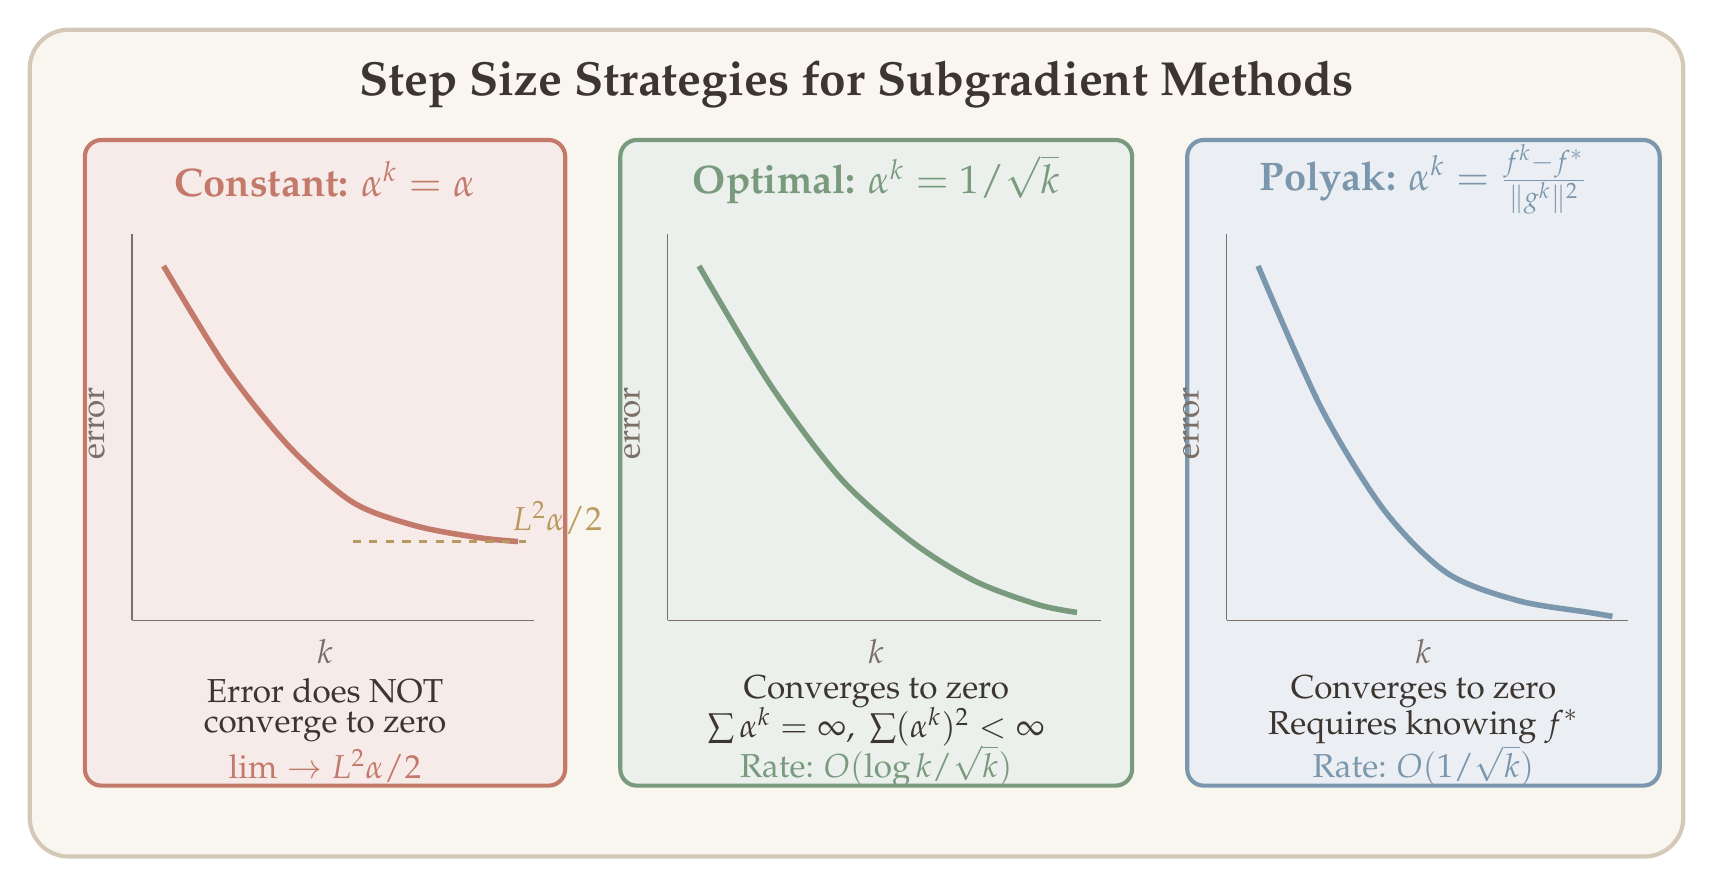
\begin{tikzpicture}[>={Stealth[length=4mm, width=3mm]}]

% Background
\fill[cream, rounded corners=14pt] (-0.5,-0.5) rectangle (20.5,10.0);
\draw[border, line width=1.5pt, rounded corners=14pt] (-0.5,-0.5) rectangle (20.5,10.0);

% Title
\node[text=dkbrown, font=\LARGE\bfseries] at (10,9.3) {Step Size Strategies for Subgradient Methods};

% --- Column 1: Constant ---
\fill[terracotta!15, rounded corners=6pt] (0.2,0.4) rectangle (6.3,8.6);
\draw[terracotta, line width=1.5pt, rounded corners=6pt] (0.2,0.4) rectangle (6.3,8.6);
\node[text=terracotta, font=\Large\bfseries] at (3.25,8.1) {Constant: $\alpha^k = \alpha$};

% Mini plot: error plateaus
\draw[wmgray, line width=0.5pt] (0.8,2.5) -- (5.9,2.5);
\draw[wmgray, line width=0.5pt] (0.8,2.5) -- (0.8,7.4);
\node[text=wmgray, font=\large] at (3.25,2.1) {$k$};
\node[text=wmgray, font=\large, rotate=90] at (0.35,5.0) {error};

% Error curve that plateaus
\draw[terracotta, line width=2pt] plot[smooth, tension=0.5] coordinates {(1.2,7.0) (2.0,5.7) (2.8,4.7) (3.6,4.0) (4.4,3.7) (5.2,3.55) (5.7,3.5)};

% Plateau line
\draw[rwgold, line width=0.8pt, dashed] (3.6,3.5) -- (5.8,3.5);
\node[text=rwgold, font=\large, right] at (5.5,3.8) {$L^2\alpha/2$};

\node[text=dkbrown, font=\large] at (3.25,1.6) {Error does NOT};
\node[text=dkbrown, font=\large] at (3.25,1.15) {converge to zero};
\node[text=terracotta, font=\large] at (3.25,0.65) {$\lim \to L^2\alpha/2$};

% --- Column 2: Decaying 1/sqrt(k) ---
\fill[sage!15, rounded corners=6pt] (7.0,0.4) rectangle (13.5,8.6);
\draw[sage, line width=1.5pt, rounded corners=6pt] (7.0,0.4) rectangle (13.5,8.6);
\node[text=sage, font=\Large\bfseries] at (10.25,8.1) {Optimal: $\alpha^k = 1/\sqrt{k}$};

% Mini plot
\draw[wmgray, line width=0.5pt] (7.6,2.5) -- (13.1,2.5);
\draw[wmgray, line width=0.5pt] (7.6,2.5) -- (7.6,7.4);
\node[text=wmgray, font=\large] at (10.25,2.1) {$k$};
\node[text=wmgray, font=\large, rotate=90] at (7.15,5.0) {error};

% Error curve that slowly decays
\draw[sage, line width=2pt] plot[smooth, tension=0.5] coordinates {(8.0,7.0) (8.9,5.5) (9.8,4.3) (10.7,3.5) (11.5,3.0) (12.3,2.7) (12.8,2.6)};

\node[text=dkbrown, font=\large] at (10.25,1.6) {Converges to zero};
\node[text=dkbrown, font=\large] at (10.25,1.15) {$\sum\alpha^k = \infty,\;\sum(\alpha^k)^2 < \infty$};
\node[text=sage, font=\large] at (10.25,0.65) {Rate: $O(\log k / \sqrt{k})$};

% --- Column 3: Polyak ---
\fill[stblue!15, rounded corners=6pt] (14.2,0.4) rectangle (20.2,8.6);
\draw[stblue, line width=1.5pt, rounded corners=6pt] (14.2,0.4) rectangle (20.2,8.6);
\node[text=stblue, font=\Large\bfseries] at (17.2,8.1) {Polyak: $\alpha^k = \frac{f^k - f^*}{\|g^k\|^2}$};

% Mini plot
\draw[wmgray, line width=0.5pt] (14.7,2.5) -- (19.8,2.5);
\draw[wmgray, line width=0.5pt] (14.7,2.5) -- (14.7,7.4);
\node[text=wmgray, font=\large] at (17.2,2.1) {$k$};
\node[text=wmgray, font=\large, rotate=90] at (14.25,5.0) {error};

% Error curve that decays faster
\draw[stblue, line width=2pt] plot[smooth, tension=0.5] coordinates {(15.1,7.0) (15.9,5.2) (16.7,3.9) (17.5,3.1) (18.4,2.75) (19.3,2.6) (19.6,2.55)};

\node[text=dkbrown, font=\large] at (17.2,1.6) {Converges to zero};
\node[text=dkbrown, font=\large] at (17.2,1.15) {Requires knowing $f^*$};
\node[text=stblue, font=\large] at (17.2,0.65) {Rate: $O(1/\sqrt{k})$};

\end{tikzpicture}
\end{document}
